\section{V9}
\subsection{C/C++ Strukturen Umsetzen}
\subsubsection{Entscheidungen}
In Assembler-Sprache ist eine Entscheidung praktisch immer in einem 2-Stufigen Ablauf umgesetzt.
\begin{itemize}
    \item Benötigte Flags ermitteln
    \item Zugehörige bedingte Sprünge ausführen
\end{itemize}

Dabei wird nach folgendem Ablauf gearbeitet:\\
\vspace{-0.5cm}
\begin{enumerate}
    \item Vergleich: Zwei Werte werden subtrahiert, dabei wird nur auf die Flags geschaut.
    \item Anhand der Flags werden dann die bedingten Sprünge ausgeführt
\end{enumerate}

\subsubsection{Analyse von Hochsprachencode und Assembly-Code}
F"ur die Bestimmung der richtigen \textit{Conditional Branch} Instruktion kann wie am folgendem Beispiel gezeigt wird vorgegangen werden:

\begin{center}
	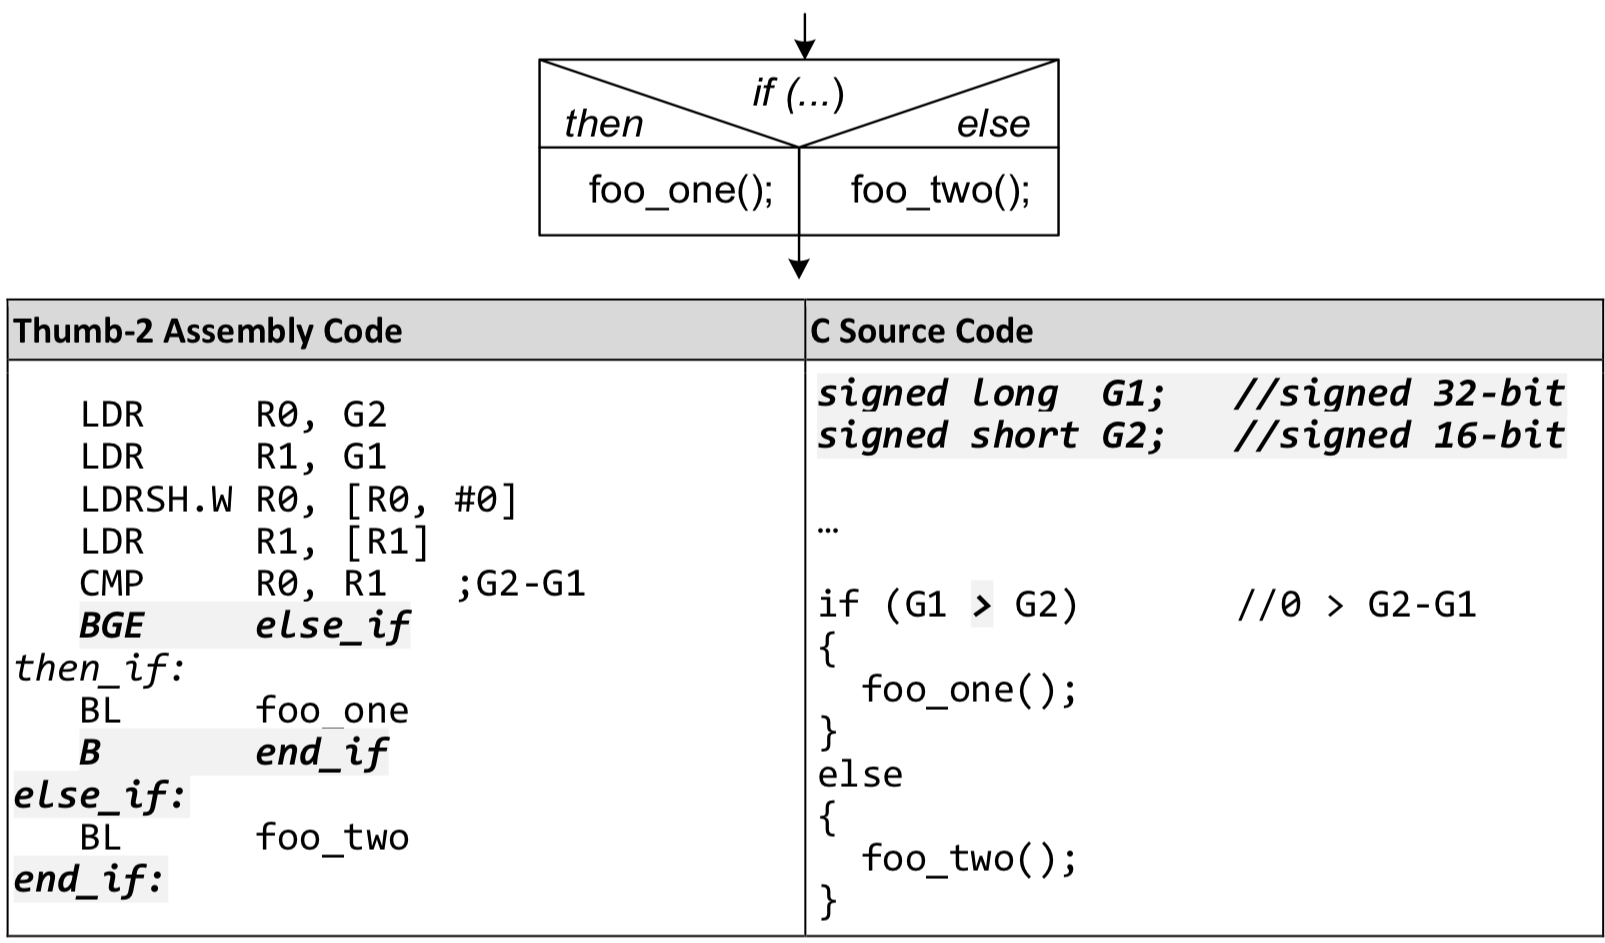
\includegraphics[width=12cm]{images/Bsp_cpp-assembly}
\end{center}

\begin{enumerate}
	\item Bestimmung des Datenformates der Variablen: \textit{signed} oder \textit{unsigned}\\
			$\Rightarrow$ Beispiel: signed
	\item Gleichung f"ur den \textit{Conditional Branch} aufstellen: \textbf{CMP Rn, Rm} entspricht Flags f"ur $Rn-Rm$\\
			$\Rightarrow$ Beispiel: $G1 > G2 \Leftrightarrow  0 > G2-G1$
\end{enumerate}
    
\begin{minipage}{9cm}
	\textbf{if-Block}\\
	F"ur einen Sprung in den if-Block w"are nun der Operator \color{red} \circled{$>$} \color{black} entscheidend.\\
	$\Rightarrow$ Conditional Branch Instruction: \textbf{BLT}\\
	Im Beispiel folgt jedoch der if-Block nach dem else-Sprung.
\end{minipage}
%
\begin{minipage}{0.5cm}
	\-\
\end{minipage}
%
\begin{minipage}{9cm}
	\textbf{else-if-Block}\\
	Die Gleichung wird zus"atzlich negiert:\\
	$0 > G2-G1$ = $\overline{0 \leq G2-G1}$\\
	F"ur einen Sprung in den else-if-Block w"are nun der Operator \color{red} \circled{$\leq$} \color{black} entscheidend.\\
	$\Rightarrow$ Conditional Branch Instruction: \textbf{BGE}
\end{minipage}

\newpage












